\begin{frame}
\frametitle{Task 3: Theory}
The radiation pattern for the co polarization according to the function 
\begin{equation}
Pattern = 10\cdot~^{10}log\left(\frac{4\pi |G_{co}(\theta, \phi_0)|^2}{P_{rad}2\eta} \right).
\end{equation}
Here the co polar radiation pattern is only considered, and is has also been normalized with respect to the radiated power. By taking the logarithm of the pattern the results will be given in [dBi] which is commonly used in antenna.

The far field patterns for the E and H plane of the far field function are defined as $|G_{co}(\theta , 0)|$ and $|G_{co}(\theta , pi/2)|$ in the H- and E- planes respectively. These patterns can be plotted in dBi as 
\begin{equation}
Pattern = 10 \cdot ~^{10}log\left(\frac{4\pi |G_{co}(\theta, \phi_0)|}{\sqrt{P_{rad}2\eta}} \right).
\end{equation}
\end{frame}



\begin{frame}
\frametitle{Task 3: Results}
\begin{columns}[c]
\column{.45\textwidth}

\begin{figure}[h]
\centering
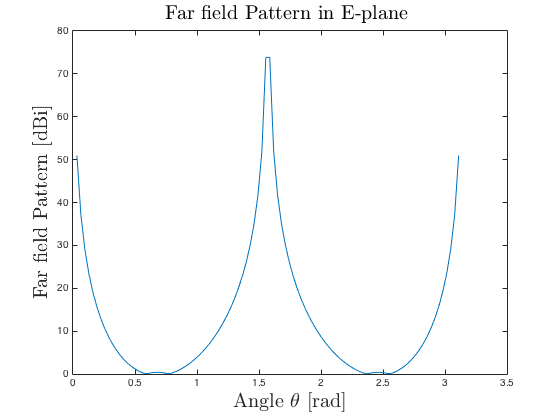
\includegraphics[scale=0.35]{/Users/marikasvensson/Documents/MATLAB/MicroProject/finished/task3/Eplane.png}
\caption{This figure shows the radiation pattern in the E-plane}
\label{task3:E-plane}
\end{figure}

\column{.5\textwidth} 
\begin{figure}[h]
\centering
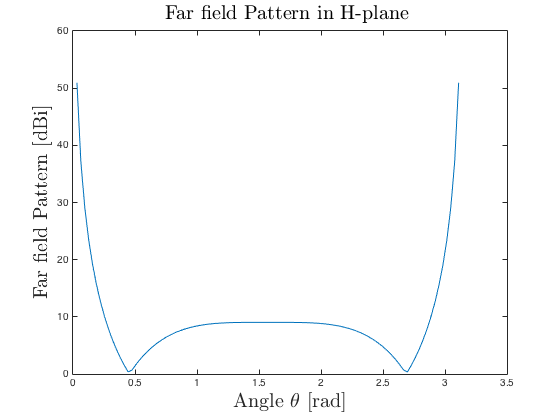
\includegraphics[scale=0.35]{/Users/marikasvensson/Documents/MATLAB/MicroProject/finished/task3/Hplane.png}
\caption{This figure shows the radiation pattern in the H-plane}
\label{task3:H-plane}
\end{figure}

\end{columns}
\end{frame}


\begin{frame}
\frametitle{Task 3: Results}
\begin{columns}[c]
\column{.45\textwidth}

\begin{figure}[h]
\centering
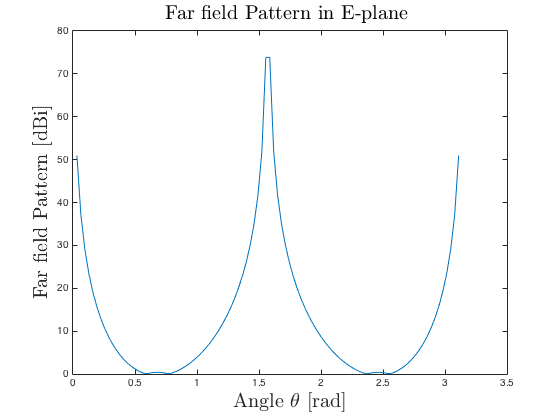
\includegraphics[scale=0.3]{/Users/marikasvensson/Documents/MATLAB/MicroProject/finished/task3/Eplane.png}
\caption{This figure shows the radiation pattern in the E-plane}
\label{task3:E-plane}
\end{figure}

\column{.5\textwidth} % Right column and width
\begin{figure}[h]
\centering
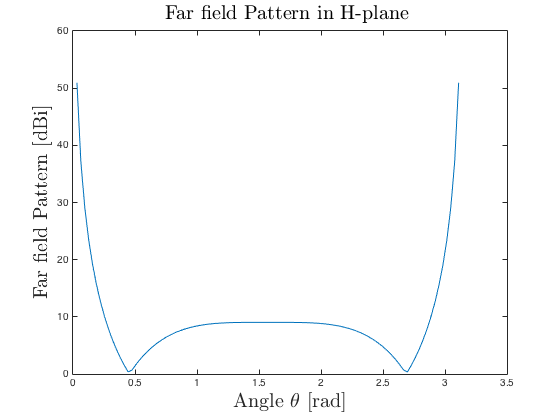
\includegraphics[scale=0.3]{/Users/marikasvensson/Documents/MATLAB/MicroProject/finished/task3/Hplane.png}
\caption{This figure shows the radiation pattern in the H-plane}
\label{task3:H-plane}
\end{figure}

\end{columns}

\end{frame}